% Options for packages loaded elsewhere
\PassOptionsToPackage{unicode}{hyperref}
\PassOptionsToPackage{hyphens}{url}
%
\documentclass[
]{book}
\usepackage{amsmath,amssymb}
\usepackage{lmodern}
\usepackage{iftex}
\ifPDFTeX
  \usepackage[T1]{fontenc}
  \usepackage[utf8]{inputenc}
  \usepackage{textcomp} % provide euro and other symbols
\else % if luatex or xetex
  \usepackage{unicode-math}
  \defaultfontfeatures{Scale=MatchLowercase}
  \defaultfontfeatures[\rmfamily]{Ligatures=TeX,Scale=1}
\fi
% Use upquote if available, for straight quotes in verbatim environments
\IfFileExists{upquote.sty}{\usepackage{upquote}}{}
\IfFileExists{microtype.sty}{% use microtype if available
  \usepackage[]{microtype}
  \UseMicrotypeSet[protrusion]{basicmath} % disable protrusion for tt fonts
}{}
\makeatletter
\@ifundefined{KOMAClassName}{% if non-KOMA class
  \IfFileExists{parskip.sty}{%
    \usepackage{parskip}
  }{% else
    \setlength{\parindent}{0pt}
    \setlength{\parskip}{6pt plus 2pt minus 1pt}}
}{% if KOMA class
  \KOMAoptions{parskip=half}}
\makeatother
\usepackage{xcolor}
\usepackage{color}
\usepackage{fancyvrb}
\newcommand{\VerbBar}{|}
\newcommand{\VERB}{\Verb[commandchars=\\\{\}]}
\DefineVerbatimEnvironment{Highlighting}{Verbatim}{commandchars=\\\{\}}
% Add ',fontsize=\small' for more characters per line
\usepackage{framed}
\definecolor{shadecolor}{RGB}{248,248,248}
\newenvironment{Shaded}{\begin{snugshade}}{\end{snugshade}}
\newcommand{\AlertTok}[1]{\textcolor[rgb]{0.94,0.16,0.16}{#1}}
\newcommand{\AnnotationTok}[1]{\textcolor[rgb]{0.56,0.35,0.01}{\textbf{\textit{#1}}}}
\newcommand{\AttributeTok}[1]{\textcolor[rgb]{0.77,0.63,0.00}{#1}}
\newcommand{\BaseNTok}[1]{\textcolor[rgb]{0.00,0.00,0.81}{#1}}
\newcommand{\BuiltInTok}[1]{#1}
\newcommand{\CharTok}[1]{\textcolor[rgb]{0.31,0.60,0.02}{#1}}
\newcommand{\CommentTok}[1]{\textcolor[rgb]{0.56,0.35,0.01}{\textit{#1}}}
\newcommand{\CommentVarTok}[1]{\textcolor[rgb]{0.56,0.35,0.01}{\textbf{\textit{#1}}}}
\newcommand{\ConstantTok}[1]{\textcolor[rgb]{0.00,0.00,0.00}{#1}}
\newcommand{\ControlFlowTok}[1]{\textcolor[rgb]{0.13,0.29,0.53}{\textbf{#1}}}
\newcommand{\DataTypeTok}[1]{\textcolor[rgb]{0.13,0.29,0.53}{#1}}
\newcommand{\DecValTok}[1]{\textcolor[rgb]{0.00,0.00,0.81}{#1}}
\newcommand{\DocumentationTok}[1]{\textcolor[rgb]{0.56,0.35,0.01}{\textbf{\textit{#1}}}}
\newcommand{\ErrorTok}[1]{\textcolor[rgb]{0.64,0.00,0.00}{\textbf{#1}}}
\newcommand{\ExtensionTok}[1]{#1}
\newcommand{\FloatTok}[1]{\textcolor[rgb]{0.00,0.00,0.81}{#1}}
\newcommand{\FunctionTok}[1]{\textcolor[rgb]{0.00,0.00,0.00}{#1}}
\newcommand{\ImportTok}[1]{#1}
\newcommand{\InformationTok}[1]{\textcolor[rgb]{0.56,0.35,0.01}{\textbf{\textit{#1}}}}
\newcommand{\KeywordTok}[1]{\textcolor[rgb]{0.13,0.29,0.53}{\textbf{#1}}}
\newcommand{\NormalTok}[1]{#1}
\newcommand{\OperatorTok}[1]{\textcolor[rgb]{0.81,0.36,0.00}{\textbf{#1}}}
\newcommand{\OtherTok}[1]{\textcolor[rgb]{0.56,0.35,0.01}{#1}}
\newcommand{\PreprocessorTok}[1]{\textcolor[rgb]{0.56,0.35,0.01}{\textit{#1}}}
\newcommand{\RegionMarkerTok}[1]{#1}
\newcommand{\SpecialCharTok}[1]{\textcolor[rgb]{0.00,0.00,0.00}{#1}}
\newcommand{\SpecialStringTok}[1]{\textcolor[rgb]{0.31,0.60,0.02}{#1}}
\newcommand{\StringTok}[1]{\textcolor[rgb]{0.31,0.60,0.02}{#1}}
\newcommand{\VariableTok}[1]{\textcolor[rgb]{0.00,0.00,0.00}{#1}}
\newcommand{\VerbatimStringTok}[1]{\textcolor[rgb]{0.31,0.60,0.02}{#1}}
\newcommand{\WarningTok}[1]{\textcolor[rgb]{0.56,0.35,0.01}{\textbf{\textit{#1}}}}
\usepackage{longtable,booktabs,array}
\usepackage{calc} % for calculating minipage widths
% Correct order of tables after \paragraph or \subparagraph
\usepackage{etoolbox}
\makeatletter
\patchcmd\longtable{\par}{\if@noskipsec\mbox{}\fi\par}{}{}
\makeatother
% Allow footnotes in longtable head/foot
\IfFileExists{footnotehyper.sty}{\usepackage{footnotehyper}}{\usepackage{footnote}}
\makesavenoteenv{longtable}
\usepackage{graphicx}
\makeatletter
\def\maxwidth{\ifdim\Gin@nat@width>\linewidth\linewidth\else\Gin@nat@width\fi}
\def\maxheight{\ifdim\Gin@nat@height>\textheight\textheight\else\Gin@nat@height\fi}
\makeatother
% Scale images if necessary, so that they will not overflow the page
% margins by default, and it is still possible to overwrite the defaults
% using explicit options in \includegraphics[width, height, ...]{}
\setkeys{Gin}{width=\maxwidth,height=\maxheight,keepaspectratio}
% Set default figure placement to htbp
\makeatletter
\def\fps@figure{htbp}
\makeatother
\setlength{\emergencystretch}{3em} % prevent overfull lines
\providecommand{\tightlist}{%
  \setlength{\itemsep}{0pt}\setlength{\parskip}{0pt}}
\setcounter{secnumdepth}{5}
\usepackage{booktabs}
\ifLuaTeX
  \usepackage{selnolig}  % disable illegal ligatures
\fi
\usepackage[]{natbib}
\bibliographystyle{plainnat}
\IfFileExists{bookmark.sty}{\usepackage{bookmark}}{\usepackage{hyperref}}
\IfFileExists{xurl.sty}{\usepackage{xurl}}{} % add URL line breaks if available
\urlstyle{same} % disable monospaced font for URLs
\hypersetup{
  pdftitle={A Minimal Book Example},
  pdfauthor={Angelo Carmignan, Gabriel Bortol, Wesley Maia},
  hidelinks,
  pdfcreator={LaTeX via pandoc}}

\title{A Minimal Book Example}
\author{Angelo Carmignan, Gabriel Bortol, Wesley Maia}
\date{2023-07-12}

\usepackage{amsthm}
\newtheorem{theorem}{Theorem}[chapter]
\newtheorem{lemma}{Lemma}[chapter]
\newtheorem{corollary}{Corollary}[chapter]
\newtheorem{proposition}{Proposition}[chapter]
\newtheorem{conjecture}{Conjecture}[chapter]
\theoremstyle{definition}
\newtheorem{definition}{Definition}[chapter]
\theoremstyle{definition}
\newtheorem{example}{Example}[chapter]
\theoremstyle{definition}
\newtheorem{exercise}{Exercise}[chapter]
\theoremstyle{definition}
\newtheorem{hypothesis}{Hypothesis}[chapter]
\theoremstyle{remark}
\newtheorem*{remark}{Remark}
\newtheorem*{solution}{Solution}
\begin{document}
\maketitle

{
\setcounter{tocdepth}{1}
\tableofcontents
}
\hypertarget{preface}{%
\chapter*{Preface}\label{preface}}
\addcontentsline{toc}{chapter}{Preface}

In this portfolio, you will find case studies covering the area of Data Science.

\hypertarget{author}{%
\chapter*{Sobre os Autores}\label{author}}
\addcontentsline{toc}{chapter}{Sobre os Autores}

\hypertarget{introduuxe7uxe3o}{%
\chapter{Introdução}\label{introduuxe7uxe3o}}

A NBA (National Basketball Association) é uma das ligas de basquete mais populares e prestigiadas do mundo, com uma rica história que se estende por 77 anos. Desde sua fundação em 1946, a NBA tem sido palco de inúmeras façanhas atléticas, rivalidades intensas e momentos memoráveis que cativaram os fãs de basquete em todo o mundo.

\hfill\break
Neste trabalho de Visualização de Dados, exploraremos um conjunto abrangente de estatísticas dos últimos 71 anos da NBA. Utilizando o Jupyter Notebook, mergulharemos nesses dados para extrair insights valiosos sobre as equipes, jogadores e padrões que moldaram a liga ao longo das décadas.

\hypertarget{objetivo}{%
\section{Objetivo}\label{objetivo}}

\hfill\break
O objetivo desta análise é investigar diversas facetas do basquete profissional, desde o desempenho das equipes até as estatísticas individuais dos jogadores. Por meio de técnicas de análise de dados e visualização, buscaremos responder a perguntas como:\\
Quais equipes dominaram a NBA ao longo dos anos? Quais jogadores tiveram as melhores performances estatísticas em diferentes épocas? Existem tendências ou padrões significativos nas estatísticas da NBA ao longo das décadas? Como o jogo evoluiu em termos de estilo de jogo, pontuação média e estilos de arremesso? Ao responder a essas perguntas, esperamos obter uma compreensão mais profunda da evolução da NBA e das dinâmicas que impulsionam o sucesso das equipes e dos jogadores ao longo do tempo. Esses insights não apenas fornecerão informações interessantes sobre a história da liga, mas também poderão ajudar a prever tendências futuras e orientar estratégias para equipes e jogadores no presente.

\hypertarget{dados}{%
\chapter{Dados}\label{dados}}

O projeto tem um conjunto de dados fornecido pelo Kaggle chamado nba.csv. NA base apresenta os dados dos jogadores de todas as temporadas de 1951 a 2022, com um total de 33330 ocorrências

\hypertarget{descriuxe7uxe3o-da-base}{%
\subsection{Descrição da base}\label{descriuxe7uxe3o-da-base}}

As colunas são descritas a seguir:

POR JOGADOR:

\begin{longtable}[]{@{}
  >{\raggedright\arraybackslash}p{(\columnwidth - 2\tabcolsep) * \real{0.0935}}
  >{\raggedright\arraybackslash}p{(\columnwidth - 2\tabcolsep) * \real{0.9065}}@{}}
\toprule()
\begin{minipage}[b]{\linewidth}\raggedright
Variável
\end{minipage} & \begin{minipage}[b]{\linewidth}\raggedright
Descrição
\end{minipage} \\
\midrule()
\endhead
Rank & A classificação do jogador (ordenado por pontos marcados a cada temporada) \\
Year & O ano da temporada (por exemplo, ``2018-19'') \\
Season Start Year & O ano de início da temporada (por exemplo, 2018) \\
Season Type & Temporada regular ou playoffs \\
Player ID & Um ID gerado para cada jogador \\
Player & O nome do jogador \\
Team ID & ID gerado para cada equipe \\
Team & A equipe do jogador na respectiva temporada \\
Games Played & Jogos disputados na respectiva temporada \\
Minutes Played & Minutos jogados na respectiva temporada \\
FG Made & Cestas de campo convertidas (Field Goals Made) \\
FG Attempts & Tentativas de cestas de campo (Field Goals Attempted) \\
FG \% & Porcentagem de acertos de cestas de campo (Field Goal Percentage) \\
3-Pt FG Made & Cestas de três pontos convertidas (3 Point Field Goals Made) \\
3-Pt FG Attempts & Tentativas de cestas de três pontos (3 Point Field Goals Attempted) \\
3-Pt FG \% & Porcentagem de acertos de cestas de três pontos (3 Point Field Goal Percentage) \\
FT Made & Lances livres convertidos (Free Throws Made) \\
FT Attempts & Tentativas de lances livres (Free Throws Attempted) \\
FT \% & Porcentagem de acertos de lances livres (Free Throw Percentage) \\
Offensive Rebounds & Rebotes ofensivos \\
Defensive Rebounds & Rebotes defensivos \\
Rebounds & Total de rebotes (ofensivos + defensivos) \\
Assists & Assistências \\
Steals & Roubos de bola \\
Blocks & Tocos (bloqueios de arremessos) \\
Turnovers & Perdas de bola (erros) \\
Personal Fouls & Faltas pessoais \\
Points Scored & Pontos marcados \\
Efficiency & Eficiência calculada como (Pontos Marcados + Rebotes + Assistências + Roubos de Bola + Tocos - Chutes de Campo Perdidos - Lances Livres Perdidos - Perdas de Bola) dividido por Jogos Disputados \\
AST/TOV & Taxa de assistências para turnovers (Assist-to-Turnover ratio) \\
STL/TOV & Taxa de roubos de bola para turnovers (Steal-to-Turnover ratio) \\
\bottomrule()
\end{longtable}

\hypertarget{explorauxe7uxe3o-dos-dados-eda}{%
\chapter{Exploração dos Dados (EDA)}\label{explorauxe7uxe3o-dos-dados-eda}}

\hypertarget{tratamento-dos-dados}{%
\section{Tratamento dos dados}\label{tratamento-dos-dados}}

Vimos que existem algum valores vazios o que é um problema para as análises que serão feitas. Vamos conferir quantas linhas do dataset existem esse tipo de dados.

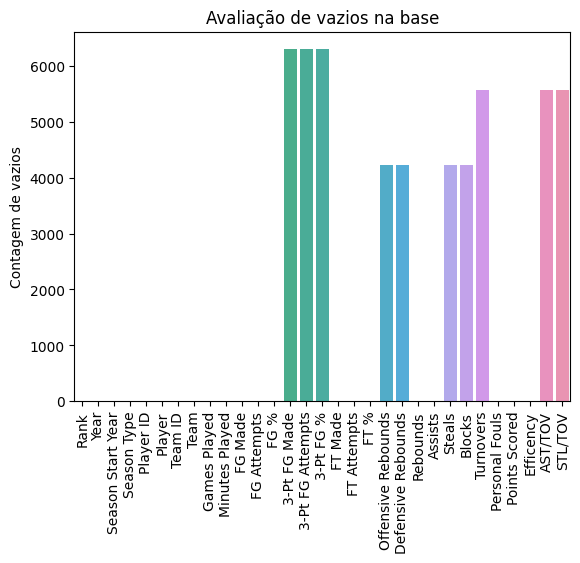
\includegraphics{imagens/1.png}

O DataFrame apresenta valores nulos em algumas colunas, como 3-Pt FG Made, 3-Pt FG Attempts, 3-Pt FG \%, Offensive Rebounds, Defensive Rebounds, Steals, Blocks, Turnovers, AST/TOV e STL/TOV. Esses valores nulos podem indicar a ausência de dados ou informações faltantes para algumas estatísticas específicas dos jogadores em determinadas temporadas.

\hfill\break
Para manter a consistência e garantir a confiabilidade da análise, optou-se por filtrar o DataFrame, excluindo as temporadas anteriores a 1978. Dessa forma, as colunas mencionadas estarão preenchidas a partir desse ano, permitindo uma análise mais completa e precisa das estatísticas dos jogadores da NBA.\\
Essa decisão foi tomada para evitar distorções nos resultados devido à ausência de dados em períodos anteriores, garantindo que a análise seja baseada em informações mais completas e recentes.

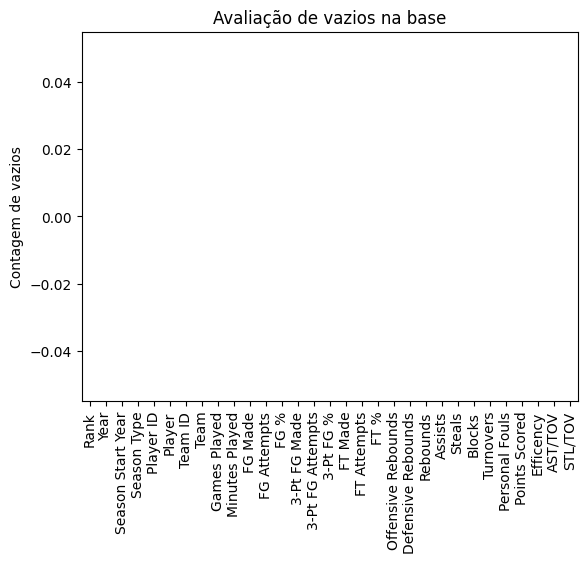
\includegraphics{imagens/2.png}

\hypertarget{primeira-pergunta-o-que-define-um-jogador-bom}{%
\subsection{Primeira pergunta: O que define um jogador bom ?}\label{primeira-pergunta-o-que-define-um-jogador-bom}}

\hfill\break
Para simplificação vamos utilizar o rank apresentado no dataset, que seriam os jogadores ordenados de acordo com a pontuação por temporada.\\
Apesar dessa rank não levar em consideração fatores defensivos, será feito uma avaliaçào se os maiores ``cestinhas'' também apresentam características defensivas acima da média.\\
A primeiro momento vamos avaliar como as informações estatísticas de cada jogador por temporada varia e como está relacionado com o rank. Para tanto será utiizado a técnica do PCA para entender melhor esse comportamento.

\hypertarget{footnotes-and-citations}{%
\chapter{Footnotes and citations}\label{footnotes-and-citations}}

\hypertarget{footnotes}{%
\section{Footnotes}\label{footnotes}}

Footnotes are put inside the square brackets after a caret \texttt{\^{}{[}{]}}. Like this one \footnote{This is a footnote.}.

\hypertarget{citations}{%
\section{Citations}\label{citations}}

Reference items in your bibliography file(s) using \texttt{@key}.

For example, we are using the \textbf{bookdown} package \citep{R-bookdown} (check out the last code chunk in index.Rmd to see how this citation key was added) in this sample book, which was built on top of R Markdown and \textbf{knitr} \citep{xie2015} (this citation was added manually in an external file book.bib).
Note that the \texttt{.bib} files need to be listed in the index.Rmd with the YAML \texttt{bibliography} key.

The RStudio Visual Markdown Editor can also make it easier to insert citations: \url{https://rstudio.github.io/visual-markdown-editing/\#/citations}

\hypertarget{blocks}{%
\chapter{Blocks}\label{blocks}}

\hypertarget{equations}{%
\section{Equations}\label{equations}}

Here is an equation.

\begin{equation} 
  f\left(k\right) = \binom{n}{k} p^k\left(1-p\right)^{n-k}
  \label{eq:binom}
\end{equation}

You may refer to using \texttt{\textbackslash{}@ref(eq:binom)}, like see Equation \eqref{eq:binom}.

\hypertarget{theorems-and-proofs}{%
\section{Theorems and proofs}\label{theorems-and-proofs}}

Labeled theorems can be referenced in text using \texttt{\textbackslash{}@ref(thm:tri)}, for example, check out this smart theorem \ref{thm:tri}.

\begin{theorem}
\protect\hypertarget{thm:tri}{}\label{thm:tri}For a right triangle, if \(c\) denotes the \emph{length} of the hypotenuse
and \(a\) and \(b\) denote the lengths of the \textbf{other} two sides, we have
\[a^2 + b^2 = c^2\]
\end{theorem}

Read more here \url{https://bookdown.org/yihui/bookdown/markdown-extensions-by-bookdown.html}.

\hypertarget{callout-blocks}{%
\section{Callout blocks}\label{callout-blocks}}

The R Markdown Cookbook provides more help on how to use custom blocks to design your own callouts: \url{https://bookdown.org/yihui/rmarkdown-cookbook/custom-blocks.html}

\hypertarget{sharing-your-book}{%
\chapter{Sharing your book}\label{sharing-your-book}}

\hypertarget{publishing}{%
\section{Publishing}\label{publishing}}

HTML books can be published online, see: \url{https://bookdown.org/yihui/bookdown/publishing.html}

\hypertarget{pages}{%
\section{404 pages}\label{pages}}

By default, users will be directed to a 404 page if they try to access a webpage that cannot be found. If you'd like to customize your 404 page instead of using the default, you may add either a \texttt{\_404.Rmd} or \texttt{\_404.md} file to your project root and use code and/or Markdown syntax.

\hypertarget{metadata-for-sharing}{%
\section{Metadata for sharing}\label{metadata-for-sharing}}

Bookdown HTML books will provide HTML metadata for social sharing on platforms like Twitter, Facebook, and LinkedIn, using information you provide in the \texttt{index.Rmd} YAML. To setup, set the \texttt{url} for your book and the path to your \texttt{cover-image} file. Your book's \texttt{title} and \texttt{description} are also used.

This \texttt{gitbook} uses the same social sharing data across all chapters in your book- all links shared will look the same.

Specify your book's source repository on GitHub using the \texttt{edit} key under the configuration options in the \texttt{\_output.yml} file, which allows users to suggest an edit by linking to a chapter's source file.

Read more about the features of this output format here:

\url{https://pkgs.rstudio.com/bookdown/reference/gitbook.html}

Or use:

\begin{Shaded}
\begin{Highlighting}[]
\NormalTok{?bookdown}\SpecialCharTok{::}\NormalTok{gitbook}
\end{Highlighting}
\end{Shaded}


  \bibliography{book.bib,packages.bib}

\end{document}
